\section{自适应 \texorpdfstring{$\lambda$}{λ}：梯度范数平衡为何没有形成稳定收益？}
\label{sec:adaptive}

\subsection{探索动机与权重学习方法}

分类与对齐损失的梯度会随训练改变，固定 $\lambda$ 未必使两项约束始终保持相近影响。本阶段借鉴 GradNorm 的梯度平衡思路\cite{chen2018gradnorm}，在共享 conv5 参数上监测两项损失的梯度范数，并学习正的适应权重。这里仅实现范数匹配控制器。

记共享参数上的梯度为 $g_{\mathrm{CE}}=\nabla_\theta\CE$、$g_G=\nabla_\theta G$，对其范数维护 decay=0.9 的指数滑动平均（EMA），以 $s=\log\lambda$ 参数化正权重，最小化
\begin{equation*}
 J_\lambda=\left(e^s\overline{\norm{g_G}_2}-\overline{\norm{g_{\mathrm{CE}}}_2}\right)^2.
 \label{eq:controller}
\end{equation*}
独立 Adam 以学习率 0.01 更新 $s$，权重裁剪在 $[10^{-4},100]$ 内；模型更新使用停止梯度的 $\lambda$。初值为 0.5，预热阶段固定权重、更新范数统计。实验覆盖 fc8 全程自适应、最后 20\% 轮次自适应，以及 conv5+fc8 第 50 轮起自适应；与相同预算的固定权重组比较。

\subsection{实验结果与训练轨迹}

表\ref{tab:lambda}同时给出最佳值与最终值。fc8 全程自适应的峰值为 54.97\%，第 50 轮为 51.32\%；固定组为 54.21\%。第 41 轮才开始学习的 fc8 最终为 53.58\%，其最佳值出现在第 37 轮，即权重学习开始之前。延迟启动没有改变这一配置的最佳记录。

\begin{table}[H]
 \centering\small
 \caption{固定与自适应权重实验。准确率单位为 \%；末次 $\lambda$ 是最后一步权重更新后的值，不同于最后一轮使用权重的均值。}
 \label{tab:lambda}
 \begin{tabular}{lrrrr}
 \toprule
 配置 & 轮数 & 最佳值 / 轮次 & 最终值 & 末次 $\lambda$\\
 \midrule
 \WeightsRows
 \bottomrule
 \end{tabular}
\end{table}

对于 conv5+fc8 的 100 轮对照，固定组第 58 轮达到 56.48\%，最终为 52.58\%；延后自适应组第 58 轮达到 55.97\%，最终为 53.58\%。自适应组的末轮多 1.01 pp，峰值则少 0.50 pp。因此，这组数据既不能被概括为所有指标都变差，也不能支持稳定改善：两种结果选择方式给出了不同方向的差值。

\begin{figure}[H]
 \centering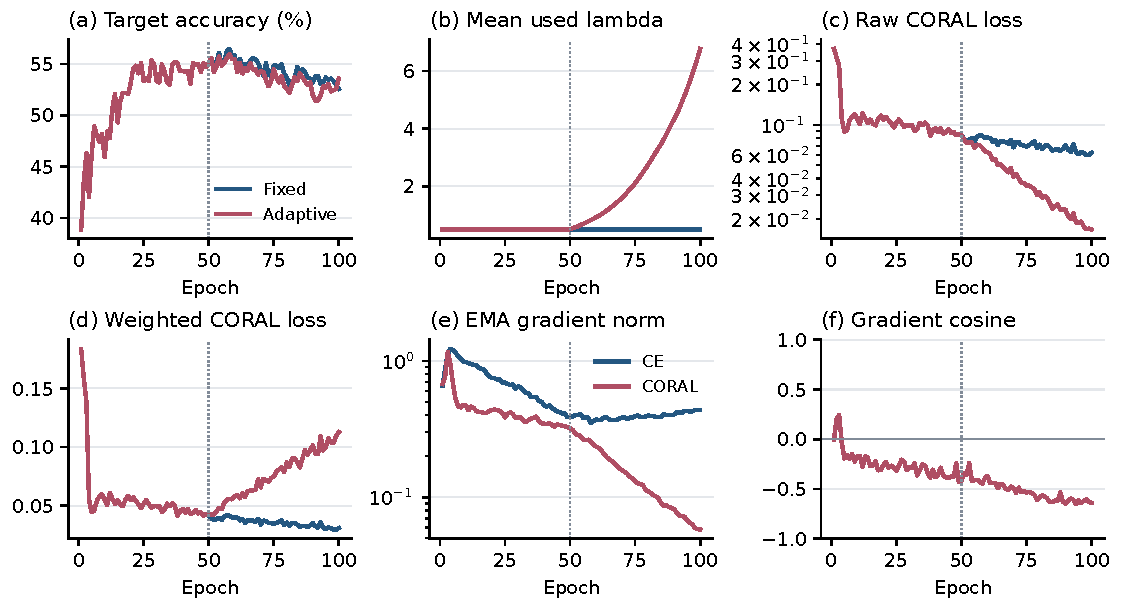
\includegraphics[width=\linewidth]{adaptive.pdf}
 \caption{conv5+fc8 固定与延后自适应的 100 轮轨迹。虚线为第 50 轮启用位置。梯度统计取自共享 conv5 参数，(e) 是范数 EMA，(f) 为逐批梯度余弦的轮均值。曲线未平滑或补点；图 (b) 为实际使用权重的轮均值。}
 \label{fig:adaptive}
\end{figure}

两组前 49 轮的分类损失、CORAL 损失与准确率在 $10^{-6}$ 容差内一致。图\ref{fig:adaptive}显示，开启自适应后，控制器不断增加权重：末次更新后 $\lambda$ 为 6.94，第 100 轮实际使用权重的均值为 6.77。原始 $G$ 从第 49 轮约 0.0853、第 50 轮 0.0837，变为第 100 轮 0.0167；与此同时，加权项没有按同样比例变小，第 100 轮 $\lambda G$ 的逐批均值为 0.11267，分类损失为 0.09619。

\subsection{失败分析：平衡了大小，没有处理方向}

\textbf{权重上升符合控制器自身的目标。}第 50 轮的平均 EMA 范数比 $\overline{\norm{g_{\mathrm{CE}}}}/\overline{\norm{g_G}}$ 约为 1.21，第 100 轮约为 7.53。随着 CORAL 梯度变小，式\eqref{eq:controller}要求更大的 $\lambda$ 才能补足范数差距。权重没有达到上界，现有记录也没有非有限优化失败；更直接的问题是控制器的目标与目标域分类质量并不等价。

\textbf{两项梯度存在方向冲突。}自适应组第 100 轮的梯度余弦均值为 $-0.641$，第 50 轮为 $-0.415$。对忽略动量与权重衰减的一次理想化梯度步，有
\begin{equation*}
 \Delta\CE\approx-\eta\left(\norm{g_{\mathrm{CE}}}_2^2
       +\lambda\langle g_{\mathrm{CE}},g_G\rangle\right).
 \label{eq:direction}
\end{equation*}
当内积为负时，提高对齐权重会抵消一部分源域分类下降方向；即使两项范数匹配，方向关系也不会因此改善。式\eqref{eq:direction}说明该控制目标遗漏了什么，但它不是目标误差变化的因果估计。实际更新还包含动量、权重衰减和其余网络参数，轮均范数与轮均余弦也不能直接代入还原每步内积。

此外，原始 CORAL 变小既可能来自有效匹配，也可能来自表示尺度变化。当前自适应实验没有保存足够的特征几何诊断，不能把图\ref{fig:adaptive}中的损失下降直接称为特征坍塌。Deep CORAL 原文关于单独优化对齐项可能出现退化解的讨论\cite{sun2016deep}提供了需要检查的方向，而不是对本次训练状态的证明。

\subsection{阶段结论与反思}

本阶段不保留这套自适应控制器作为有效改进方案。它提高了原始对齐目标的优化压力，却没有带来稳定的分类收益；\textbf{把范数匹配当作优化目标，需要同时检查梯度方向与表示几何}。只在共享 conv5 上测量的统计也不能代表所有层的更新关系。
